\begin{figure}[H]
    \centering
    \begin{subfigure}{0.45\textwidth}
        \centering
        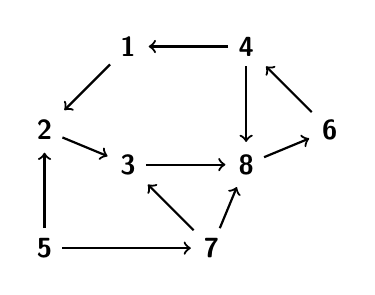
\begin{tikzpicture}[->,shorten >=1pt,auto,node distance=1.5cm,
                            thick,main node/.style={font=\sffamily\bfseries}]

        % Define vertices
        \node[main node] (1) {1};
        \node[main node] (2) [below left of=1] {2};
        \node[main node] (3) [below of=1] {3};
        \node[main node] (4) [right of=1] {4};
        \node[main node] (5) [below left of=3] {5};
        \node[main node] (6) [below right of=4] {6};
        \node[main node] (7) [below right of=3] {7};
        \node[main node] (8) [right of=3] {8};

        % Draw edges
        \path[every node/.style={font=\sffamily\small}]
            (1) edge (2)
            (2) edge (3)
            (3) edge (8)
            (4) edge (1)
            (4) edge (8)
            (5) edge (2)
            (5) edge (7)
            (6) edge (4)
            (7) edge (3)
            (7) edge (8)
            (8) edge (6);

        \end{tikzpicture}
        \caption{Graph 2}
        \label{fig:graph2}
    \end{subfigure}
    \begin{subfigure}{0.45\textwidth}
        \centering
        \begin{tikzpicture}[level distance=1.25cm,
                            level 1/.style={sibling distance=1.25cm},
                            level 2/.style={sibling distance=1cm},
                            thick,main node/.style={circle,draw,font=\sffamily\bfseries}]

        % Define vertices
        \node[main node] (R) {R}
            child {node[main node] (1) {1}}
            child {node[main node] (2) {2}}
            child {node[main node] (3) {3}}
            child {node[main node] (B) {B}
                child {node[main node] (4) {4}}
                child {node[main node] (6) {6}}
                child {node[main node] (8) {8}}
            };
        \node[main node, right=1.5cm of R] (5) {5};
        \node[main node, right=1.25cm of 5] (7) {7};
        \end{tikzpicture}

        \caption{SCC Tree of Graph 2} 
        \label{fig:scc_tree2}      
    \end{subfigure}
    \caption{Graph 2 and its SCC-trees}
    \label{fig:graph2_scc_tree}
\end{figure}
 